\documentclass{proc}
\usepackage{url}
\def\UrlBreaks{\do\/\do-}
\usepackage{graphicx}
\usepackage{epstopdf}
\usepackage{eso-pic}
\usepackage{picture}
\linespread{1.2}

\begin{document}

\title{GlassBox: Fault-Tolerant Host Monitoring on Commodity Operating Systems}

\author{Brett Jia \hspace{1em} Jennifer Bi}

\maketitle

\section*{Abstract}

In modern computer systems, administrators, developers, and users often desire to monitor their operating systems for usage metrics, such as filesystem usage, CPU utilization, RAM utilization, and others. In other cases, systems administrators and developers may be interested in monitoring log files on production machines to gauge the health and execution of live applications. Monitoring can be done through automated software that report metrics to a metrics aggregator, or through a user manually running certain tools that probe the operating system for data. In either case, the system could be at risk of damage and compromise from buggy or malicious software and user negligence or error. To address this problem, we present an approach to running host monitoring tools in containers with a read-only view of the surrounding system, guaranteeing fault tolerance and protection to the host operating system.

\section*{1. Introduction}

Despite the best efforts of software designers and system administrators, a major weakness of system administration and system monitoring is the reliance on bug-free software and perfect user execution. While some system monitoring tools such as \texttt{ps} do not require elevated privileges and rely on reading deprivileged virtual filesystem objects exposed by the operating system kernel via the \texttt{procfs} mount, other tools such as \texttt{lsof} require superuser privileges to display full metrics on a system's open file descriptors by reading protected files in the same \texttt{procfs} mount. Especially for the case of tools requiring superuser privileges, any system administration or system monitoring task could potentially be destructive to the host system through malicious software or user error if incorrect commands and arguments are executed, resulting in the expenditure of hours and money to restore the system and its contents to a state prior to disaster.

Aside from monitoring of host system data and statistics, often system administrators and developers alike desire to monitor interesting files on a machine's filesystem for tracing the execution of a running application or troubleshooting software. Files such as \texttt{/var/log/messages} and application runtime logs provide a wealth of information about the health and execution of the system and live applications running on the host, and these logs can be used in a chain of standard Unix commands (such as \texttt{grep} and \texttt{sort}) to provide useful metrics and analysis. Similar to the risks of running system monitoring tasks, even accessing log files directly on the machine (whether using a privileged user or not) can jeopardize the health and stability of the host and the applications running on the host by accidentally crashing applications or starving the host of resources by spending too much computing resources on log file analysis.

An early solution to the problem of fault tolerance is to utilize virtual machines to guarantee isolation between processes \cite{garfinkel2003terra}. However, while virtual machines can indeed be used to provide an isolated environment for untrusted code execution \cite{wen2012virtualization}, recent performance comparisons between hypervisor-based virtualization and container-based (i.e. lightweight or kernel-based) virtualization show that virtual machines exhibit more overhead with certain workloads when compared to kernel-supported container mechanisms \cite{felter2014docker, morabito2015hypervisors}.

Instead of fault tolerance through hardware virtualization by way of virtual machines, recent work has emphasized ensuring fault tolerance through operating system virtualization \cite{soltesz2007container}. An early approach to operating system virtualization introduces a kernel interposition method to restrict an application's access to certain system calls (syscalls), as implemented in Janus \cite{goldberg1996janus} and later in MBOX \cite{kim2013mbox}. Other sandboxing mechanisms have been introduced, including new system calls to create kernel-supported process isolation called jails \cite{kamp2000jails}, new filesystem tools leveraging \texttt{mount} and \texttt{chroot} to restrict filesystem access \cite{prevelakis2001fmac}, namespace isolation to create kernel-supported process containers \cite{biederman2006namespaces, menage2007containers}, and control groups (\textit{cgroups}) to limit resource consumption of a group of processes \cite{menagecgroups}.

Modern containers combine these operating system virtualization approaches to create lightweight isolated execution contexts. The industry standard choice for Linux container technology is Docker, which combines Linux \textit{cgroups}, \textit{namespaces}, \textit{capabilities}, and more using its custom container runtime, \textit{libcontainer} \cite{hykes2014libcontainer}. With the formation of the Open Container Initiative (OCI) in 2015 \cite{opencontainerinitiative}, the design and construction of container platforms became standardized with OCI's \textit{runtime-spec} and \textit{image-spec}, providing a framework for distributors to develop their own cross-compatible container implementations.

In our research, we present \textit{GlassBox}, a system to provide fault-tolerance and fault-containment semantics to host monitoring processes on commodity Linux operating systems. \textit{GlassBox} addresses the problems of host stability and fault tolerance that arise from executing buggy or compromised system tools and from user negligence and error when performing system administration tasks and application log monitoring through the use of modern container technologies. In the following sections, we first present background on containers and existing container technologies, then discuss a theoretical view of the host resources a fault-tolerant host monitoring system should allow access to and the resources the system should protect, then discuss the prototype architecture and implementation of \textit{GlassBox}, and close with preliminary performance benchmarks and future work.

\section*{2. Containers}

Linux supports the creation of isolated filesystem environments through \texttt{chroot} jails and \texttt{mount} namespaces. While \texttt{chroot} changes the root filesystem directory for a process, \texttt{mount} namespaces allow for flexibility of what directory the process sees as the filesystem root and security of the overall filesystem on the host. Bind mounts (\texttt{mount} command with the \texttt{--bind} option) in particular make a subset of a host's filesystem visible at a second mount point \cite{bindmount}, with the option of mounting it as ``read-only.'' This kind of ``symbolic link'' allows for a specific view of the filesystem namespace. By bind mounting the root directory or \texttt{/proc}, host information becomes readable by a jailed process otherwise closed off from the filesystem. Indeed, bind mounts can currently be used with Docker containers to provide visibility to certain files on the host filesystem while keeping the containers' stong isolation guarantees \cite{dockerdoc}.

Host-monitoring applications isolated in read-only filesystems may also need a place to temporarily store the output of its monitoring. \texttt{tmpfs} can be used to store temporary data in RAM rather than on disk. Furthermore, the size can be limited to prevent a host-monitoring program from consuming too much memory. When combined with Docker, a \texttt{tmpfs} mount is persisted in host memory while the container runs, and removed when a container stops.

Linux also supports syscall filtering via \texttt{seccomp-bpf} filters, which are used in conjunction with other container primitives to implement containerization in Docker, LXC, etc. Currently, the container runtime \textit{runC} (built on its predecessor \textit{libcontainer} \cite{hykes2014libcontainer}) uses \texttt{seccomp-bpf} to perform syscalls interposition \cite{opencontainerinitiative}. The rule-based filtering of existing \textit{seccomp-bpf} in Linux, however, does not allow for more advanced access control policy validation or syscall emulation \cite{seccompuserspace}.

Commercial container solutions such as Docker and rkt offer pre-built networking options to faciliate networking connectivity between the container and the host \cite{dockernetworking, rktnetworking}. The two general categories of network connectivity offered are \textit{host} and \textit{container}, both built on the network separation properties provided by Linux network namespaces. \textit{Host} network configurations set up the container to share the same network namespace as that of the calling process, effectively giving the container the same network access and network configuration as the parent process. \textit{Container} network configurations create a separate network namespace for the container, separating its connectivity from the network namespace of the parent process. In \textit{container} network configurations, a network bridge and virtual ethernet devices are used to connect the container's network with the host, effectively exposing the container as a new ``host'' connected to the host machine.

CPU and memory usage can also be restricted in existing container solutions through the use of Linux capabilities and \textit{cgroups} \cite{dockerconstraints}. As \textit{cgroups} function to group a set of processes under the same ``control group'' for broad resource control and process management \cite{menagecgroups}, container implementations such as Docker use \textit{cgroups} to fine-tune the memory and CPU-time allowances of the group of processes running in a container. Additionally, Linux capabilities can be used to give the container permission to modify its process scheduler directly in the host kernel, such as setting \textit{nice} values or use the Linux \textit{realtime} process scheduler.

\section*{3. Fault-Tolerant Host Monitoring}

We postulate that an ideal fault-tolerant host monitoring system should observe the following two characteristics:
\begin{enumerate}
    \item The system should be able to accurately view the host's state, both volatile (e.g. in-memory) and persistent (e.g. on-disk), as needed by the information the system is monitoring.
    \item The system's execution, both in normal and abnormal circumstances, must guarantee that stability of the host machine is maintained.
\end{enumerate}

An accurate view of the host's state is required for the host monitoring system to be useful. For example, the \texttt{top} program, which monitors system memory and CPU usage by process, requires access to volatile information to function correctly (in this case, the \texttt{/proc} virtual file system). It is easy to imagine that the \texttt{top} tool would not function correctly or be nearly as useful if \texttt{/proc} did not exist, or if reading from \texttt{/proc} yielded incorrect or invalid data.

On the other hand, a strong guarantee that the monitoring system's execution maintains the stability of the host machine is required to ensure fault-tolerance. We define the property of maintaining a host's \textit{stability} as ``preventing any modification of volatile and persistent data or usage of computing resources that could, now or in the future, alter the execution or responsiveness of the host or applications on the host.'' In other words, the monitoring system should ensure that it accesses memory and storage outside of the monitor in a strictly read-only fashion, should not send any signals or messages to existing processes, and should not starve the host of shared resources.

% discuss tradeoffs of accurate monitoring and fault-tolerance

\section*{4. GlassBox Implementation}
\begin{figure}
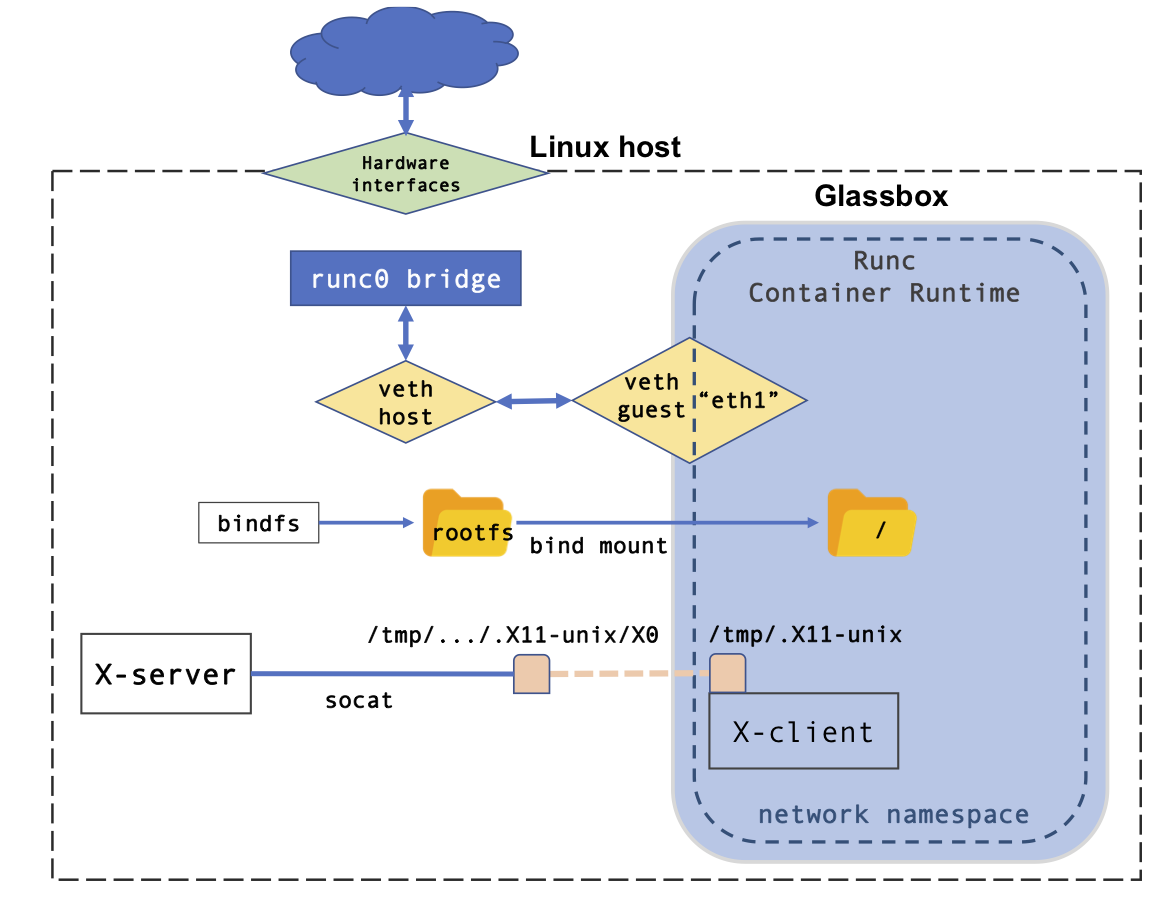
\includegraphics[width=0.5\textwidth]{architecture}
\caption{Architecture diagram}
\end{figure}
%Include information about container implementation

GlassBox is implemented on top of a runC container to provide an accurate, read-only view of the host state, including commonly monitored information such as CPU load, process information, memory usage, and network traffic. By read-only, we mean that changes to the host state either fail (for example, sending a kill signal to a process running on the host) or ephemeral (for example, writing to a file). Practically, read-only behavior guarantees the stability of the host. GlassBox uses bindfs/FUSE filesystem, OverlayFS filesystem, Linux tmpfs temporary file storage, the \texttt{iptables} utility, and Linux namespaces and capabilities, and the runC container runtime.

\subsection*{Root filesystem}
We found that most host-monitoring tools, from simple commands that ship with Linux to complex graphical tools, all rely on a few Linux interfaces such as the \texttt{/proc} and \texttt{/sys} directories. By read-only bind-mounting the host's root to the container root, we make the host root filesystem available at these two mount points. Given access to the root file system, many tools like \texttt{top} can successfully collect statistics on the host. 

Host-monitoring tools may write temporary log files to the filesystem. GlassBox adds an ephemeral layer via tmpfs and overlay filesystems to enable the these host-monitoring tools to function properly, while also ensuring that the writes to the host filesystem are ephemeral. Figure 2 shows the setup. The \texttt{overlay\_home} directory is the writeable upper directory. The \texttt{overlay\_work} directory is a writeable layer created in tmpfs. The \texttt{overlay\_home} is mounted on top of the bind-mounted root filesystem, to present a unified view of the upper directory (which is writeable) and the underlying root directory tree (which is read-only). Writing to the overlay layer is eleting from the lower directory creates a 'whiteout'
%%% more details

\subsection*{Networking}
GlassBox provides networking to containers via a bridge network. Each GlassBox instance has a network namespace to present the container its own network stack, routes, firewall rules, and network devices. Before the first container instance is launched, GlassBox creates the bridge network on the host and assigns an IP address. For each container, a Linux Virtual Ethernet (veth) device pair is created in the host network namespace. The host end of the pair is added to bridge network in the host network namespace, and the guest end is moved to the guest network namespace and added as an interface. The veth pair is a full duplex link, and thus acts as a tunnel between the bridge network and the guest network namespace. By default, the guest end of the veth pair is the only exposed interface in the container. Each guest-end of the veth pair is associated with an IP \texttt{192.168.10.<container id>}, where the id is a random integer between 0-255. 
We create read-only behavior using \texttt{iptables} to restrict network packets. The \texttt{netfilter/iptables} utility uses a series of tables, each of which define firewall rules to filter or transform packets. To allow GlassBox to listen on the host's network traffic, we apply an iptables rule (\texttt{TEE}) that clones the packet and redirects it to our gateway IP. To prevent GlassBox processes from sending packets to (and potentially spamming) the host, we specify the iptables rule (\texttt{DROP}) to drop outgoing packets. Thus, when multiple containers are connected to the same bridge network via veth pairs, each container cannot communicate with the host, nor with any other container. 

Finally, runC provides configuration options for Linux capabilities to be set in a container. We set two capabilities by default, texttt{CAP\_NET\_ADMIN} for listing all network interfaces, and \texttt{CAP\_NET\_RAW} to use raw sockets, which enable monitoring of network traffic.

One limitation of the networking setup is that the interfaces seen by GlassBox (for example, by running \texttt{ip addr} are different from those seen by the host. We consider this discrepancy acceptable, since practically, host monitoring tools such as \texttt{tcpdump, Wireshark} are interested in the network traffic rather than the the interfacs themselves. Since \texttt{TEE} clones the network packets, the IP source/destination appearing in packet captures still reflect the host interfaces. 


\subsection*{X11 and Graphical Tool Support}





\begin{figure}
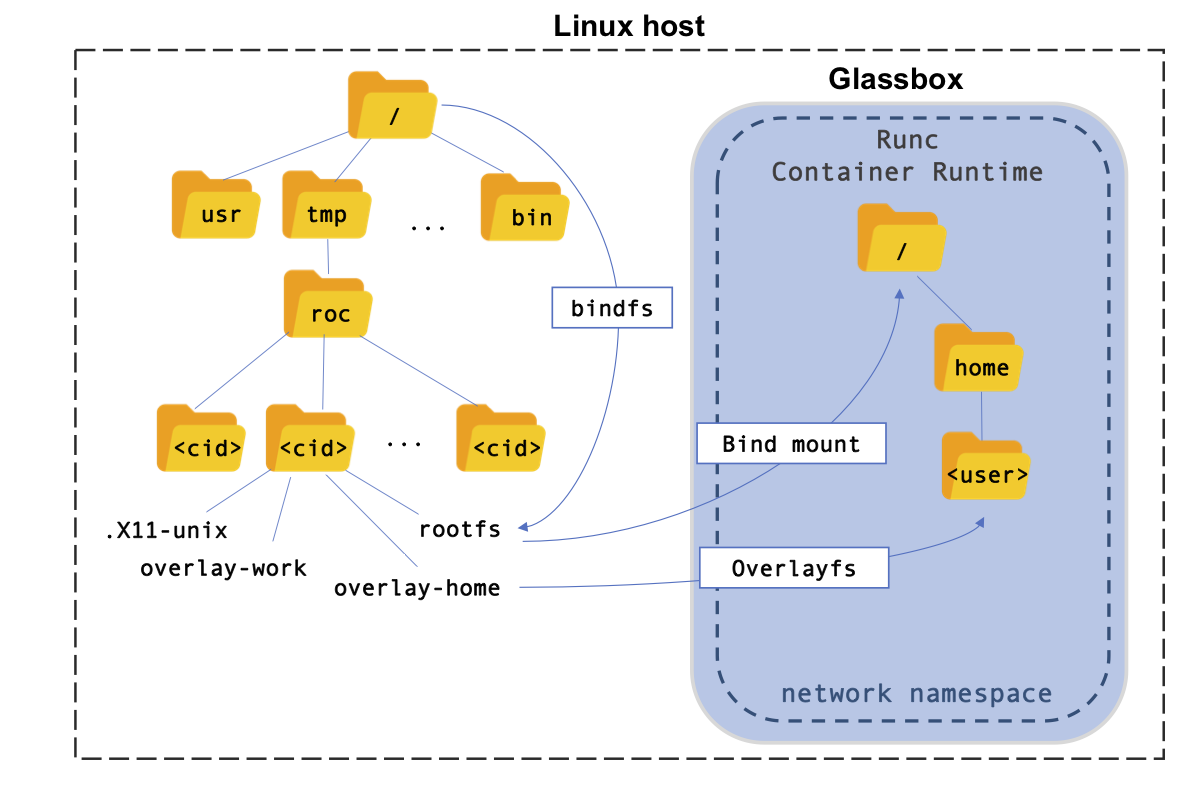
\includegraphics[width=0.5\textwidth]{fs_diagram}
\caption{Filesystem setup}
\end{figure}

GlassBox relaxes the isolation provided by containers like Docker. For example, despite having a separate pid namespace, GlassBox exposes host process information via the \texttt{/proc} directory. Therefore, as a proof-of-concept it made sense to extend runC to implement our read-only isolation, rather than building our own container. Additionally, the runC component of GlassBox can be easily swapped out for a different container runtime such as LXC or rkt.
\section*{4. Evaluation}

We evaluated GlassBox on a range of host-monitoring and application performance monitoring tools. This includes Linux commands like \texttt{top} or \texttt{free}, more complex utilities like \texttt{sysstat} \cite{sysstat}, remote monitoring tools like \textit{GKrellM} \cite{gkrellm}, and graphical tools like \textit{Wireshark}, \textit{Cacti} \cite{cacti} and \textit{Nagios} \cite{nagios}. We also ensured that standard Unix tools (e.g. \texttt{awk}, \texttt{grep}, \texttt{vim}, \texttt{md5sum}) work correctly.
\subsubsection*{4.2 Required Software}

We will use the same Linux distribution on development VMs as those in the CLIC lab. Our other software is also open-source or free: standard system tools that ship with Linux, \textit{Cacti}, \textit{Nagios}, \textit{GKrellM}, \textit{sysstat}, and \textit{Docker}.

\section*{5. GlassBox Performance}

%Include information about GlassBox experimental setup, including using tini as a lightweight userspace reaper to accurately track the container's process tree (since bindfs daemonizes)

We hypothesize that monitoring tools will be able to run successfully and access host information in our container, while incurring some small overhead. The overhead will likely be due to syscall interposition and setup/teardown related to managing read access to host filesystems. We hypothesize that monitoring directly on the host do not get the benefits of protection of host resources, while monitoring from inside a Docker container is possible, but requires additional configuration for read-only access, and even then may be too restrictive for certain tools to function correctly.

\section*{6. Future Work}

%Include future work

\section*{7. Conclusions}

%Include conclusions, mention there is more work to be done to improve the container and add additional features

\bibliographystyle{abbrv}
\bibliography{extended-abstract}

\clearpage

\section*{Appendix A}

\AddToShipoutPicture*{
    \put(.5\paperwidth,.5\paperheight){\makebox(0,0){\includegraphics[scale=1]{memdata.eps}}}
}

\end{document}
